\chapter{Generative Machine Learning}
In the first chapter we said that in this course we would consider \textit{``machines that think, that learn and that create''}, following Herbert Simon’s definition of autonomous and adaptive systems. Until now we have focused on the first two points, discussing reinforcement learning and how we can build agents that take actions given a representation of the state. It is now time to move on to machines that \textit{create}.

Can machines even be creative? We will now see a few examples of generative models but let us always keep in mind the definition of \textbf{creativity} given by Margaret Ann Boden, a research professor of cognitive science at the University of Sussex: \textit{``Creativity can be defined as the ability to generate novel, and valuable, ideas. Valuable, here, has many meanings: interesting, useful, beautiful, simple, richly complex, and so on. Ideas covers many meanings too: not only ideas as such (concepts, theories, interpretations, stories), but also artifacts such as graphic images, sculptures, houses, and jet engines. Computer models have been designed to generate ideas in all these areas and more''}.

\section{Generative modeling}
\textbf{Generative models} are a class of statistical models that allow for the generation of new data instances. Given a set of data instances $X$ and a set of labels $Y$, they capture the joint probability $p(X,Y)$, or just $p(X)$ if there are no labels\footnote{From \url{https://developers.google.com/machine-learning/gan/generative}}. An example of such models are ones that predict the next word in a sequence. 

These models, however, tend to generate data that is just a variation of the one that has been used to train them, not meeting the novelty criterion we have presented earlier on. Given a dataset $\boldsymbol{X}$, produced according to an unknown distribution $p_{data}$, we want to create a generative model $p_{model}$ that can be used to generate samples that look like they were drawn from $p_{data}$ while also being different enough to be considered novel.

\subsection{Deep Dream}
Deep Dream is a computer vision program created by Alexander Mordvintsev, Christopher Olah and Mike Tika in 2015. It uses a deep convolutional neural network to find and enhance patterns in images creating a dream-like appearance in deliberately over-processed images\footnote{From \url{https://en.wikipedia.org/wiki/DeepDream}}.

While interpretability is still an open question in the deep learning field, image classifiers do not suffer from the same issue. Each layer, in fact, extracts higher and higher-level features of the images in order to make its classification decision. This can be exploited by means of a technique known as \textit{gradient ascent in input space}: we apply gradient \textit{descent} to the value of the input image of a convolutional neural network so as to maximize the response of a specific filter, starting from a blank input image. The resulting input image will be one that the chosen filter is maximally responsive to.

The same technique is used in Deep Dream: one or more layers are chosen, and an input is built so as to maximize the excitement from those layers. If we give the network an actual image as an input instead of noise, the network will then modify the image to maximize the response of the layers we chose, outputting the ``hallucinogenic'' results Deep Dream is known for.

\begin{figure}
    \centering
    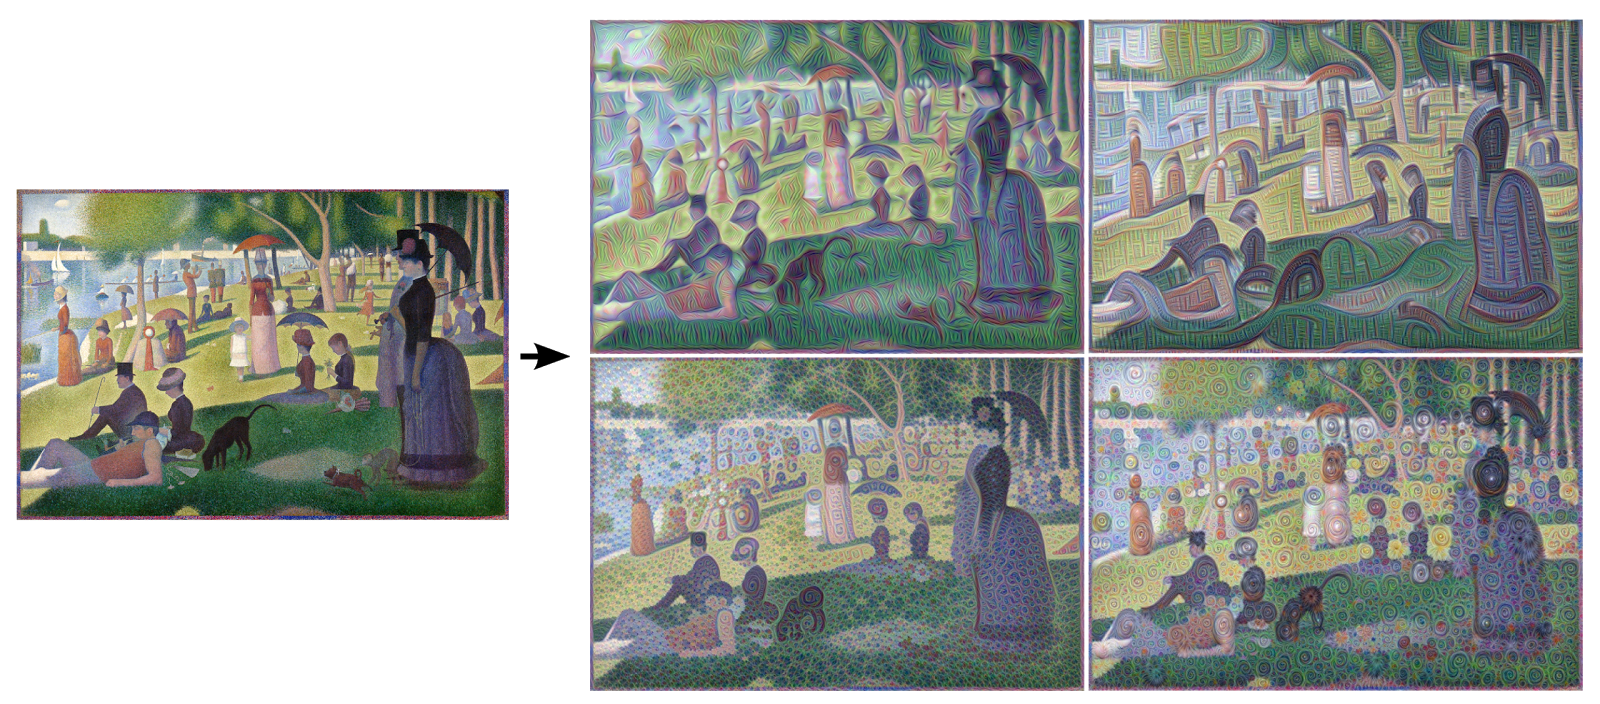
\includegraphics[scale=0.25]{Images/Chapter 10/deepdream.png}
    \caption{\textit{``A Sunday Afternoon on the Island of La Grande Jatte''} reimagined by DeepDream}
    \source{GoogleAI Blog}
    \label{fig:ch10-deepdream}
\end{figure}

\subsection{Generative Adversarial Networks}
Performing gradient ascent on a certain input image is not the only way for machines to create something original. Many of us will have probably come across the website ``This Person Does Not Exist''\footnote{\url{https://thispersondoesnotexist.com/}}, where we can see pictures of people that have been generated by a neural network called StyleGAN2.

GAN stands for Generative Adversarial Network, a class of machine learning frameworks designed by Ian Goodfellow and his colleagues in 2014 \cite{goodfellow2014generative}. They are made up of two neural networks: a \textbf{generative network}, responsible for generating candidates and a \textbf{discriminative network} that evaluates them. The objective of the generative network is to fool the discriminative network into believing that the image was part of the ground truth data used to train it\footnote{From: \url{https://en.wikipedia.org/wiki/Generative_adversarial_network}}.

\begin{figure}
    \centering
    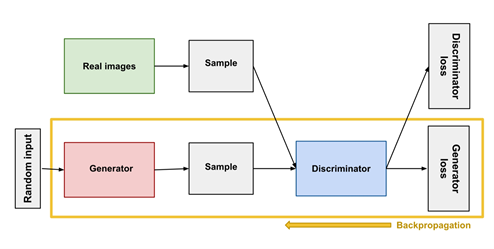
\includegraphics{Images/Chapter 10/gan.png}
    \caption{Structure of a Generative Adversarial Network}
    \source{Google Developers website}
    \label{fig:ch10-gan}
\end{figure}

\subsection{Text generation}
Neural networks can also generate text with great results. The latest and greatest example in these types of networks is GPT-3 (Generative Pre-trained Transformer 3), an autoregressive language model developed by OpenAI and published in May 2020. Trained with 175 billion parameters, it has been able to generate text with a quality so high that it difficult to distinguish from that written by a human.